%---------change this every homework
\def\yourid{yl4df}
\def\collabs{mw5ew}
\def\sources{list any sources, e.g.\ Cormen, et al, Introduction to Algorithms}
% NOTE: To specifically cite your sources, include your bibliography.bib file from
% homework 0 when LaTeXing your document (or upload it to Overleaf with this document)
% and then uncomment the penultimate last two lines of this file to display the
% bibliography.
% -----------------------------------------------------
\def\duedate{Monday, April 27 at 11p}
\def\duelocation{via Collab}
\def\hnumber{9}
\def\course{{cs4102 - algorithms - spring 2020}}%------
%-------------------------------------
%-------------------------------------

\documentclass[10pt]{article}
\usepackage[colorlinks,urlcolor=blue]{hyperref}
\usepackage[osf]{mathpazo}
\usepackage{amsmath,amsfonts,graphicx}
\usepackage{latexsym}
\usepackage[top=1in,bottom=1.4in,left=1.25in,right=1.25in,centering,letterpaper]{geometry}
\usepackage{color}
\definecolor{mdb}{rgb}{0.1,0.6,0.4} 
\definecolor{cit}{rgb}{0.05,0.2,0.45} 
\pagestyle{myheadings}
\markboth{\yourid}{\yourid}
\usepackage{clrscode}
\usepackage{url}
\usepackage{tabularx,booktabs}
\usepackage{framed}
\usepackage{tikz}
\usetikzlibrary{arrows}
\newcolumntype{Y}{>{\centering\arraybackslash}X}

\newenvironment{proof}{\par\noindent{\it Proof.}\hspace*{1em}}{$\Box$\bigskip}
\newcommand{\handout}{
   \renewcommand{\thepage}{Homework \hnumber~-~\arabic{page}}
   \noindent
   \begin{center}
      \vbox{
    \hbox to \columnwidth {\sc{\course} \hfill}
    \vspace{-2mm}
       \hbox to \columnwidth {\sc due \MakeLowercase{\duedate} \duelocation\hfill {\Huge\color{mdb}H\hnumber(\yourid)}}
      }
   \end{center}
   \vspace*{1mm}
   \hrule
   \vspace*{1mm}
    {\footnotesize \textbf{Collaboration Policy:} You are encouraged to collaborate with up to 4 other students, but all work submitted must be your own {\em independently} written solution. List the computing ids of all of your collaborators in the comments at the top of the tex file. {\color{cit} You \textbf{are} permitted to collaborate through online tools such as Google Docs, interactive whiteboards, Google Meet, Google Hangouts, Zoom, Skype, etc, however you \textbf{must} limit written/typed details to high-level algorithm design.  Each person is responsible for taking those ideas and turning them into pesudocode and a writeup. Do \textbf{NOT} copy and paste from shared documents, which includes re-typing verbatim or trying to disguise text that you are essentially copying.  Over-collaboration of that form is fairly easy to detect with plagiarism tools.} {\color{red}\textbf{Do not seek published or online solutions, including pseudocode, for this assignment.}} If you use any published or online resources (which may not include solutions) when completing this assignment, be sure to cite them. Do not submit a solution that you are unable to explain orally to a member of the course staff. Any solutions that share similar text/code will be considered in breach of this policy. Please refer to the syllabus for a complete description of the collaboration policy.
   \vspace*{1mm}
    \hrule
    \vspace*{2mm}
    \noindent
    \textbf{Collaborators}: \collabs\\
    \textbf{Sources}: \sources}
    \vspace*{2mm}
    \hrule
    \vskip 2em
}
\newcommand{\solution}[1]{\medskip\noindent\textbf{Solution:}#1}
\newcommand{\bit}[1]{\{0,1\}^{ #1 }}
%\dontprintsemicolon
%\linesnumbered
\newtheorem{problem}{\sc\color{cit}problem}
\newtheorem{extra}{\sc\color{cit}extra credit}
\newtheorem{practice}{\sc\color{cit}practice}
\newtheorem{lemma}{Lemma}
\newtheorem{definition}{Definition}
\newtheorem{theorem}{Theorem}
\newcommand{\answer}[1]{\color{blue}\hfill\break\\\noindent\textbf{#1}\color{black}\hfill\break}
\newcommand{\points}[1]{\normalfont{[#1 points]}}

\newcommand{\Z}{\mathbb{Z}} % This might be useful for Integers!

\begin{document}
\thispagestyle{empty}
\handout

%----Begin your modifications here


\begin{problem}Curbside Takeout \points{20}\end{problem}

    IKEA is growing in popularity across the US, however their stores are only found in a handful of larger metropolitan areas.  While their main product is furniture, they have become known for their signature meatballs.  To increase profits and make their delicious food more accessible, they have decided to open local take-out only IKEA Curbside restaurants in towns across the country.  Restaurant storefronts are expensive to rent and maintain, so they are happy with customers needing to drive at most to the next town over to get their IKEA meatball fix.  Specifically, their goal is that every town in America either has an IKEA Curbside, or its neighboring town has an IKEA Curbside.

Given a graph representing the towns and roads between them (representing the towns being neighbors), the \emph{Curbside} problem is to decide whether $k$ IKEA Curbside locations can be placed in order to ensure that each town or its neighbor has an IKEA Curbside location.  Show that \emph{Curbside Takeout} is NP-Complete.

Note: You are not being asked to explicitly solve the \emph{Curbside Takeout} problem; you are only required to show that it is NP-Complete.
\begin{proof}
First, we prove it is NP. Suppose we are given a witness $I$ consisting of $k$ towns. Then for each town in $I$, mark the town as visited and check every incident roads. Mark all neighbor towns as visited. After looping through all towns in $I$, if all towns in G are visited, then the solution works. Otherwise, it fails. The verification process takes $O(E+V)$ which is in polynomial time, so the problem is NP.

Second, we prove it is NP-Hard. We prove this by showing k-vertex cover reduces to Curbside Takeout in polynomial time. Suppose we are given a graph $G$. We construct another graph $G'$ in such a way: 
\begin{enumerate}
    \item Keep all vertices and edges the same as they are in $G$.
    \item For each edge $\{u, v\}$, do not change it. Add a new node $w$ and connect $w$ with $u$ and $v$. That is, we create a triangle for each original edge.
\end{enumerate}
Then we claim the k-vertex cover problem for $G$ has solution $S$ of size at most $k$ if and only if Curbside Problem for $G'$ has solution $C$ of size $k$.

Forward direction: Suppose $S$ is a k-vertex cover for $G$. Take a arbitrary node $v \in G'$. If $v$ is a original node, then either $v \in S$, or the node $u$ connected by edge $\{u, v\}$ is in $S$. If $v$ is a newly added node, then it connects with two original nodes. As we argued above, at least of of these two original nodes is in $S$, so the newly added node $v$ has neighbor nodes in $S$. Thus, every node in $G'$ is either in $S$ or has neighbors in $S$. $S$ is the solution of Curbside Takeout for $G'$.

Backward direction: Suppose $C$ solves Curbside Takeout for $G'$. Then we look at the newly added nodes $w \in C$. We know $w$ only connects $u$ and $v$. If either $u$ or $v$ is in $C$, then we could safely eliminate $w$ from $C$ to form a new set $C'$, because the edge $\{u, v\}$ is already covered by $u$ or $v$. If neither $u$ nor $v$ is in $C$, we can replace $w$ by either $u$ or $v$ to form new set $C'$ and get edge $\{u, v\}$ covered. Thus, graph $G$ has the vertex cover $C'$ of size at most $k$.

Since we prove the both directions, the reduction is correct. The instance-mapping and solution-mapping takes polynomial time because we just loop through the graph to add or remove nodes. Since k-vertex cover is NP-Hard, then Curbside Takeout is NP-Hard.

Since Curbside Takeout is NP and NP-Hard, we conclude that Curbside Takeout is NP-Complete.

\end{proof}
\begin{problem} European Summer Vacation \points{20}\end{problem}

You and a friend are heading to Europe for the summer (hopefully!).  You have completed your packing list, and combined, you need to bring $n$ items in total, with the weights of the items given by $W = (w_1, \ldots, w_n)$.  Your goal is to divide the items between your suitcases such that the difference in weight between them is at most $t$. We formally define the problem below: 

\begin{framed}
  \noindent
  \textsc{Suitcase}: Given a sequence of non-negative weights $W = (w_1, \ldots, w_n)$ and a target weight difference
  $t$, can you divide the items among you and your friend such that the weight difference between suitcases is at most $t$?
\end{framed}
  
  Show that the \textsc{Suitcase} problem defined above is $\mathsf{NP}$-complete (namely, you should
  show that $\textsc{Suitcase} \in \mathsf{NP}$ and that \textsc{Suitcase} is $\mathsf{NP}$-hard). For this
  problem, you may use the fact that the \textsc{SubsetSum} problem is $\mathsf{NP}$-complete:

  \begin{minipage}[t]{\linewidth}
  \begin{framed}
    \textsc{SubsetSum}: Given a sequence of non-negative integers $a_1, \ldots, a_n$
    and a target value $t$, does there exist
    a subset $S \subseteq \{ 1, \ldots, n \}$ such that $\sum_{i \in S} a_i = t$?
  \end{framed}
  \end{minipage}

\begin{proof}
First, we show SUITCASE is NP by giving a polynomial time verifier. Suppose we are given a way of dividing. The verification can be done by summing up all weights on me and on my friend, and checking whether the difference is at most $t$. The summation and comparison clearly takes polynomial time, so SUITCASE is NP.

Second, we show SUITCASE is NP-Hard by showing SUBSETSUM $\leq _p$ SUITCASE. Suppose we are given a sequence $A$ of non-negative integers $a_1, \ldots, a_n$ and a target value $t$. The total sum of the sequence $A$ is $T$. Then we add a item $b$ weighing $T-2t$ to $A$ to construct a new sequence $A'$ with total sum $2T-2t$. To establish the correctness of reduction, we need to prove that SUBSETSUM has solution for $(A,t)$ if and only if SUITCASE has solution for $(A',0)$.

Forward Direction: Suppose we have solution of SUBSETSUM that there exists a subset in $A$ with sum of $t$. Then we add a item weighing $T-2t$ to the subset, so we a have new subset with sum of $T-t$. Since the total sum of $A'$ is $2T-2t$, we successfully divides $A'$ such that weight difference between two parts is at most 0. 

Backward Direction: Suppose we have solution of SUITCASE that divides $A'$ such that weight difference between two parts is at most 0. This means each part has weight $T-t$. Now the item $b$ weighing $T-2t$ will be in either part. For the part where $b$ is in, the remaining items has weight $(T-t)-(T-2t)=t$. The subset containing these remaining items gives the solution for SUBSETSUM. We successfully find a subset of $A$ with sum of $t$.

Since we prove the both directions, the reduction is correct. The instance-mapping takes polynomial time because we just add one item. The solution-mapping takes polynomial time because we just remove that item. Thus, we have SUBSETSUM $\leq _p$ SUITCASE. Since SUBSETSUM is NP-Hard, then SUITCASE is NP-Hard.

Since SUITCASE is NP and NP-Hard, we conclude that SUITCASE is NP-Complete.
\end{proof}
\newpage
\begin{problem} Lecture Review Questions \points{20}\end{problem}

    \begin{enumerate}
        \item Briefly explain the difference between the Edmonds-Karp and Ford-Fulkerson algorithms for Max Flow.  Why does this difference reduce the runtime for Edmonds-Karp?
            \answer{EK chooses augmenting path with fewest hops, whereas FF does not have restriction on augmenting path. In order words, EK is FF using BFS to find augmenting path. 
            \\This difference guarantees at least one path was saturated at each loop, so we loop $|V||E|$ times instead of $|f|$ times.} % put your answer inside this command

        \item Define ``augmenting path.''  Provide an example from the residual graph below by listing the nodes in path order.

   \begin{center}
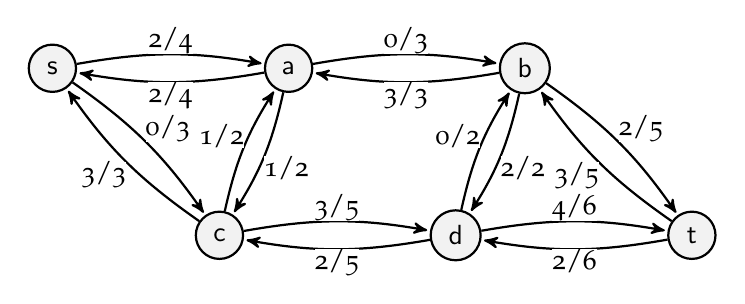
\begin{tikzpicture}[->,>=stealth',shorten >=1pt,auto,node distance=3cm,
  thick,main node/.style={circle,fill=gray!10,draw,
  font=\sffamily,minimum size=6mm}]

  \node[main node] (s) {s};
  \node[main node] (a) [right of=s] {a};
  \node[main node] (c) [below right of=s] {c};
  \node[main node] (b) [right of=a] {b};
  \node[main node] (d) [right of=c] {d};
  \node[main node] (t) [below right of=b] {t};

  \path[every node/.style={
        fill=white,inner sep=0pt,outer sep=0pt}]
    (s) edge [bend left=10] node[] {2/4} (a)
        edge [bend left=10] node[] {0/3} (c)
    (a) edge [bend left=10] node[] {0/3} (b)
        edge [bend left=10] node[] {2/4} (s)
        edge [bend left=10] node[] {1/2} (c)
    (b) edge [bend left=10] node[] {2/2} (d)
        edge [bend left=10] node[] {3/3} (a)
        edge [bend left=10] node[] {2/5} (t)
    (c) edge [bend left=10] node[] {1/2} (a)
        edge [bend left=10] node[] {3/5} (d)
        edge [bend left=10] node[] {3/3} (s)
    (d) edge [bend left=10] node[] {4/6} (t)
        edge [bend left=10] node[] {2/5} (c)
        edge [bend left=10] node[] {0/2} (b)
    (t) edge [bend left=10] node[] {3/5} (b)
        edge [bend left=10] node[] {2/6} (d);
  {}
\end{tikzpicture}
   \end{center}

            \answer{Augmenting path is a path from source to sink that using only edges with positive capacity and has no cycle. Example: s, a, c, d, t} % put your answer inside this command

        \item Briefly explain the reduction from the Vertex Disjoint Paths problem to Edge Disjoint Paths and why that reduction correctly solves Vertex Disjoint Paths.
            \answer{Make two copies of each node, one connected to incoming edges and the other connecting to outgoing edges. Connect two copies by one edge for each node. Compute EDP on the new graph. Collapse corresponding nodes in the result to get the solution for VDP. \\
            There is only one edge connecting in-vertex and out-vertex, so computing EDP on new graph will guarantee paths with vertex disjoint.} % put your answer inside this command

        \item What must be proven to show that a problem is in NP-Complete?
            \answer{It is NP: give a poly time verifier;\\
            It is NP-Hard: show that another NP-Hard problem reduces to it in polynomial time.} % put your answer inside this command

        \item Which of the following would show that problem $A$ is worst-case $\Theta(n \log n)$?  No justification is needed.
            \begin{itemize}
                \item[a) ] Reduce problem $A$ to comparison-based sorting in linear time
                \item[b) ] Reduce comparison-based sorting to problem $A$ in linear time
            \end{itemize}
            \answer{b} % put your answer inside this command

    \end{enumerate}

%%%%%%%%%%%%%%%%%%%%%%%%%%%%%%%%%%%%%%%%%%%%%%%%%%%%%%%%%%%%%%%%%%%%%%%%%%%%%%
% EXTRA CREDIT OPPORTUNITY
\newpage
\noindent
   \begin{center}
      \vbox{
          \hbox to \columnwidth {\hfill {\sc \Huge\color{mdb}EC3(\yourid)}}
      }
   \end{center}
   \vspace*{1mm}
   \hrule
   \vspace*{1mm}
    {\footnotesize \textbf{Extra Credit Instructions:} For each of the next three written homeworks (HW6, HW7, HW9), you will be given an extra credit problem, with the opportunity to replace one homework at the end of the course.  Combined, the extra credit portions are worth $60$ points---the same as one normal homework assignment.  Each Extra Credit portion (EC1, EC2, EC3) will be combined into one \emph{optional} replacement homework, meaning that the total scored out of all $60$ extra credit points will replace your lowest homework grade for the semester.  Note: this extra credit will \textbf{not} be applied to this homework (HW\hnumber).  To make the most of this opportunity, you should commit to solving \textbf{all} extra credit portions for the next three homework assignments.}
   \vspace*{1mm}
    \hrule
    \vspace*{2mm}
    \noindent
    {\footnotesize Since the extra credit is optional, no office hours will be provided to aid in solving the additional \emph{optional} problems.}
    \vspace*{2mm}
    \hrule
    \vskip 2em

\begin{extra} Insert/Delete/Min Data Structure \end{extra}

Prove whether there exists a data structure where the operations $\mathtt{INSERT}$ (which inserts a given element into the data structure), $\mathtt{DELETE}$ (which removes a given element from the data structure, should it be present), and $\mathtt{MIN}$ (which returns the minimum element from the data structure) require $O(1)$ worst-case time each.

\begin{proof}
Proof by contradiction. Suppose there exists such a data structure that INSERT, DELETE, and MIN takes constant time. Then we could design a comparison-based sorting algorithm based on such data structure. Suppose the input size is $n$. Initialize two instances of such data structure $p$ and $q$. INSERT all values which need to be sorted into $p$. This step takes $O(n)$ because INSERT takes $O(1)$ for each element. Perform MIN on $p$, INSERT the returned min value in $q$, and DELETE the min value from $p$. Repetitively run the three steps above until MIN returns nothing ($p$ is empty). The sorted values are in $q$. Then the algorithm takes $O(1)+O(1)+O(1)$ in worst case for each item in $p$. Since input size is $n$, this sorting algorithm takes $O(n)$ in worst case. However, we know the worst-case lower-bound time complexity for comparison-based sorting is $\Omega (n\log n)$. This leads to contradiction, so there is no such a data structure that INSERT, DELETE, and MIN takes constant time.
\end{proof}


% Bibliography - uncomment the next two lines to cite your sources!
%\bibliographystyle{plain}
%\bibliography{bibliography}
\end{document}

